\documentclass[a4paper]{article}
\usepackage{exercise}
%um nur aufgaben zu zeigen
\renewcommand{\title}{Aufgabenseminar\\ Himmelsmechanik}
\newcommand{\titleh}{Aufgabenseminar Himmelsmechanik}

%\usepackage[noanswer]{exercise} 
\usepackage{../images/preamble}
\usepackage{rotating}
\usetikzlibrary{decorations.pathmorphing}
\usetikzlibrary{decorations.markings}
\usetikzlibrary{arrows}
\usetikzlibrary{shapes.geometric}
\newcommand{\midarrow}{\tikz \draw[-triangle 90] (0,0) -- +(.02,0);}
\usepackage{xcolor}
%\usepackage{draftwatermark}
%\SetWatermarkText{\textsc{Entwurf}}
%\SetWatermarkScale{6}
%\SetWatermarkColor{red!30}

\pagestyle{fancy}
\fancyhead[L]{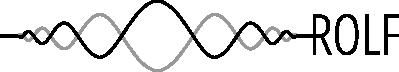
\includegraphics[width=2cm]{../images/logo_scaled.pdf}}
\fancyhead[R]{\textsc{\titleh}}



\begin{document}
	\vspace*{-1cm}
	\parbox{4cm}{\vspace{-0.2cm}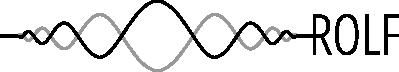
\includegraphics[width=5cm]{../images/logo_scaled.pdf}}
	\parbox{10.6cm}{\setstretch{2.0} \centering{ \huge \textsf{\title
			}}\\\url{pankratius.github.io/rolf}
			 }
		\vspace{0.5cm}
	
	

\thispagestyle{empty}
\begin{framed}
	\noindent
	\scriptsize
	
	Gravitationskraft $\mathbf{F} = \frac{mMG}{r^2}\hat{\mathbf{r}}$; Gravitationspotential $U\left(r\right) = -\frac{mMG}{r}$; Gesamtenergie auf einer elliptischen Flugbahn $E = \frac{mMG}{2a}$; Fläche einer Ellipse $A = \pi a b$; für Punkt auf Ellipse bleibt Summe der Abstände zu den Brennpunkten konstant,  Runge-Lenz-Vektor $\mathbf{\varepsilon} = \frac{\mathbf{L}\times \mathbf{v}}{GmM} + \hat{\mathbf{r}} = \mathrm{const.}$\\
	Kepler I: Bewegung von HK auf Kegelschnitten ($r\left(\varphi\right) = \frac{p}{1+\varepsilon \cos \varphi}$, mit $p = \ell^2/\Gamma m^2$ und $\varepsilon^2 = 1 + 2E^2\ell^2/\Gamma^2 m^3 $), Brennpunkt im Schwerpunkt; Kepler II: Radiusvektor überschreitet gleiche Flächen in gleichen Zeiten; Kepler III: für zwei Bahnen gilt $\nicefrac{T^2}{T^2} = \nicefrac{a_1^2}{a_2^3}$\\
	 \noindent\rule{1\textwidth}{0.4pt}
	wichtige Größen: Abstand von Schwerpunkt ($r$), Gravitationskraft($\mathbf{F}$), Gravitationspotential ($U\left(r\right)$), Energie ($E\left(r\right)$), Drehimpuls ($\mathbf{L}$), Betrag des Drehimpulses ($\ell$), Umlaufzeit ($T$), große Halbachse ($a$), kleine Halbachse ($b$), Masse eines Körpers im gegebenen Gravitationsfeld ($m$), Masse des Gravitationsfeld erzeugenden Körpers ($M$), Gravitationskonstante ($G$)\\
	Wo es sinnvoll ist, ersetzen wir $GM$ durch eine neue Konstante, $\Gamma$\\
	 \noindent\rule{1\textwidth}{0.4pt}
	Taylor-Näherung: $f\left(x\right) \approx f\left(x_0\right) + \frac{df}{dx}|_{x=x_0} \left(x-x_0\right)$ für $x\approx x_0$.
	
	
\end{framed}

\noindent

\begin{minipage}[b]{0.65\textwidth}
\begin{Exercise}[title = Polygon, origin = P. Gnädig, difficulty = 2, label = polygrav]
	Wir betrachten ein regelmäßiges n-Eck, bei dem an jeder Ecke eine Masse $m$ sitzt. Wie bewegt sich das System, wenn nur die Gravitationskraft zwischen den Körpern wirkt? Wie viel Zeit (in Abhänigkeit von $n$) vergeht, bis das System seinen Endzustand erreicht hat? 
\end{Exercise}
\end{minipage}
\begin{minipage}[b]{0.35\textwidth}
	\centering
	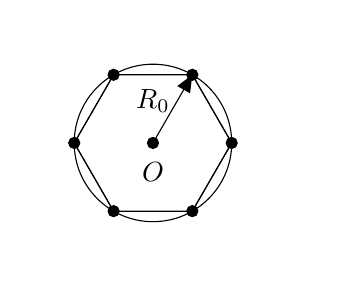
\begin{tikzpicture}[line cap=round,line join=round,>=triangle 45,x=1.0cm,y=1.0cm]
	\clip(-1.0911274272504616,-0.595261736026898) rectangle (2.4959243296533993,2.330040817448145);
	\draw(0.,0.) -- (1.,0.) -- (1.5,0.8660254037844387) -- (1.,1.7320508075688776) -- (0.,1.7320508075688779) -- (-0.5,0.8660254037844395) -- cycle;
	\draw (0.,0.)-- (1.,0.);
	\draw (1.,0.)-- (1.5,0.8660254037844387);
	\draw (1.5,0.8660254037844387)-- (1.,1.7320508075688776);
	\draw (1.,1.7320508075688776)-- (0.,1.7320508075688779);
	\draw (0.,1.7320508075688779)-- (-0.5,0.8660254037844395);
	\draw (-0.5,0.8660254037844395)-- (0.,0.);
	\draw(0.5,0.866025403784439) circle (1.cm);
	\draw [->] (0.5,0.866025403784439) -- (1.,1.7320508075688776);
	\begin{scriptsize}
	\draw [fill=black] (0.,0.) circle (2.0pt);
	\draw [fill=black] (1.,0.) circle (2.0pt);
	\draw [fill=black] (1.5,0.8660254037844387) circle (2.0pt);
	\draw [fill=black] (1.,1.7320508075688776) circle (2.0pt);
	\draw [fill=black] (0.,1.7320508075688779) circle (2.0pt);
	\draw [fill=black] (-0.5,0.8660254037844395) circle (2.0pt);
	\draw [fill=black] (0.5,0.866025403784439) circle (2.0pt);
	\end{scriptsize}
	\node at (0.5,1.4){$R_0$};
	\node at (0.5,0.5){$O$};
	\end{tikzpicture}
\end{minipage}
\begin{Answer}[ref = polygrav]
	Aus Symmetriegründen heben sich die nicht-radialen Teile der wirkenden Gravitationskräfte auf, sodass alle $n$ Massen sich zum Mittelpunkt des Polygons, $O$, bewegen. Dabei muss die polygonform erhalten bleiben. Weil die Abhängigkeit Körperabstand-Gravitationskraft aber nicht-linear ist, ist die Bewegung nicht gleichmäßig beschleunigt. Vielmehr sollte die Beschleunigung größer werden, je geringer der Körperabstand ist.\\
	Um nun die Zeit $T$ auszurechnen, bis die Körper im Punkt $O$ kollidieren, kann man zuerst die Kraft auf eine der Massen $m$ ausrechnen. Diese ist gegeben durch die Summe der Radialteile aller  Gravitationskräfte der anderen $n-1$ Körper, also, wenn der Radius des Polygons gerade $R$ ist,
	\begin{equation}\label{polygrav:f}
		F = Gm \sum_{i= 1}^{n-1}\frac{m \sin\left(\frac{\pi}{i}\right)}{\left(2R  \sin\left(\frac{\pi}{i}\right)\right)^2} = \frac{Gm}{R^2}\cdot \underbrace{ \frac{m}{4}\sum_{i=1}^{n-1} \frac{1}{\sin \frac{\pi}{i}}}_{:= M_n}.
 	\end{equation}
 	Die Kraft ist also so, als würde sich der Körper im Gravitationsfeld eines stationären Körpers mit der Masse $M_n = \frac{m}{4}\sum_{i=1}^{n-1} \frac{1}{\sin \frac{\pi}{i}}$ bewegen.\\
 	Diese Bewegung kann man jetzt als Bewegung entlang einer Ellipse ohne kleiner Halbachse, und mit großer Halbachse $\frac{R_0}{2}$ auffassen. Die Zeit, die dann bis zum Zusammensturz benötigt wird, entspricht genau der halben Periode $\nicefrac{T_e}{2}$. \\
 	Diese kann man über das dritte Keplersche Gesetz aus der entsprechenden Periode $T_k$ für eine Kreisbahn mit Radius $R_0$ ausrechen, wobei $F_g = F_{rad}$ benutzt wird:
 	\begin{equation}\label{polygrav:tc}
 		\frac{GmM_n}{R_0^2}  = m R\underbrace{\left(\frac{2\pi}{T_k}\right)^2}_{=\omega ^2} \Rightarrow T_k = 2\pi\sqrt{\frac{R_0^3}{GM_n}}.
 	\end{equation}
 	Mit dem dritten Keplerschen Gesetz folgt dann
 	\begin{equation}
 	\boxed{	\left(\frac{T_e}{T_k}\right)^2 = \left(\frac{\nicefrac{R_0}{2}}{R_0}\right)^3 \Rightarrow T_e = \pi \sqrt{\frac{R_0^3}{8GM_n}}.}
 	\end{equation}
\end{Answer}
 
\begin{Exercise}[title = Ballistische Rakete, origin = J. Kaalda, difficulty =3, label = cmellipse]
	Eine Rakete wird vom Nordpol der Erde (Radius $R$, Masse $M$) mit der ersten kosmischen Geschwindigkeit\footnote[2]{Das ist die Geschwindigkeit, mit der ein Körper eine stabile Kreisbahn über der Erdoberfläche haben kann.} gestartet, sodass sie am Äquator landet. 
	\Question Wie groß ist die große Halbachse $a$ der Flugbahn?
	\Question Was ist der größte Abstand $h$ der Rakete von der Erdoberfläche?
	\Question Wie lang ist die Flugzeit $T$ der Rakete?
\end{Exercise}
\begin{Answer}[ref = cmellipse]
	\begin{figure}[h]
		\centering
		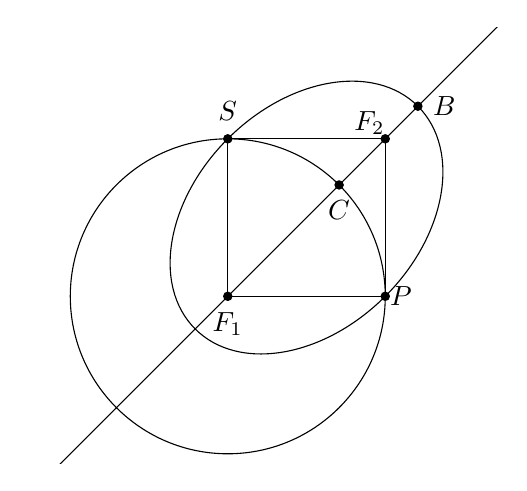
\begin{tikzpicture}[line cap=round,line join=round,>=triangle 45,x=1.0cm,y=1.0cm]
\clip(-2.541266947042949,-2.117285434822983) rectangle (3.440995527238834,3.4115693078693945);
\draw (0.,2.) -- (2.,2.) -- (2.,0.) -- (0.,0.) -- cycle;
\draw(0.,0.) circle (2.cm);
\draw [domain=-2.541266947042949:6.440995527238834] plot(\x,{(-0.--1.*\x)/1.});
\draw [rotate around={45.:(1.,1.)}] (1.,1.) ellipse (2.cm and 1.4142135623730951cm);
\draw (0.,2.)-- (2.,2.);
\draw (2.,2.)-- (2.,0.);
\draw (2.,0.)-- (0.,0.);
\draw (0.,0.)-- (0.,2.);
\begin{scriptsize}
\draw [fill=black] (0.,0.) circle (1.5pt);
\draw [fill=black] (0.,2.) circle (1.5pt);
%\draw [fill=black] (1.,1.) circle (1.5pt);
\draw [fill=black] (2.,2.) circle (1.5pt);
\draw [fill=black] (2.,0.) circle (1.5pt);
\draw [fill=black] (1.414213562373095,1.414213562373095) circle (1.5pt);
\draw [fill=black] (2.414213562373095,2.414213562373095) circle (1.5pt);
\end{scriptsize}

\node at (0,-0.35) {$F_1$};
\node at (0,2.35) {$S$};
\node at (1.8,2.2) {$F_2$};
\node at (1.4142,1.1) {$C$};
\node at (2.75,2.4142) {$B$};
\node at (2.2,0) {$P$};
\end{tikzpicture}
		\caption{Skizze der Flugbahn}
		\label{fig:cmellsk}
	\end{figure}
	\Question Die erste kosmische Geschwindigkeit $v_0$ kann man am einfachsten durch das Gleichsetzen von  Radial- und Gravitationskraft errechnen
	\begin{equation*}\label{cmellipse:vo}
		\frac{GMm}{R^2} = \frac{mv_0^2}{R} \Rightarrow v_0 = \sqrt{\frac{\Gamma}{R}}.
	\end{equation*}
	Die Gesamtenergie beim Abschuss ist damit gegeben durch
	\begin{equation*}
		E = \frac{mv_0^2}{2} - \frac{\Gamma m}{R} = -\frac{\Gamma m}{2R}
	\end{equation*}
	Damit können wir die große Halbachse $a$ ausrechnen, weil wir ja wissen, wie die beiden zusammenhängen
	\begin{equation}\label{cmellipse:sma}
	\boxed{
		E = -\frac{\Gamma m}{2a} = -\frac{\Gamma m}{2R} \Rightarrow a = R.}
	\end{equation}
	Das kann man sich auch daran überlegen, dass eine Rakete, die mit der ersten kosmischen Geschwindigkeit in einer Kreisbahn um die Erde gestartet wird, am Anfang die gleiche kinetische Energie haben muss (das haben wir ja in der Aufgabenstellung so definiert) und gleichzeitig aber auch die gleiche potentielle Energie hat. Weil die große Halbachse aber nur eine Funktion der Gesamtenergie des Systems ist, müssen beide Bahnen die gleiche große Halbachse haben, was im Fall der Kreisbahn ja offensichtlich $R$ ist, also $a = R$.
 	\Question Wir wissen, dass einer der beiden Brennpunkte $F_1$ der Erdmittelpunkt sein muss (1. Keplersches Gesetz). Die Distanz des anderen Brennpunkts vom Erdmittelpunkt finden wir über die Ellipseandefinition. Für alle Punkte $P$ auf dem Ellipsenumfang gilt für die Abstände von den Brennpunkten $F_1$ und $F_2$
	\begin{equation}\label{cmellipse:edef}
	\overline{F_1P} + \overline{F_2P} = 2a,
	\end{equation}
	wobei $a$ die große Halbachse ist, die wir ja in \eqref{cmellipse:sma} ausgerechnet haben.\\
	Aus Symmetriegründen müssen die beiden Brennpunkte nun auf einer Breite von $\frac{\pi}{4}$ liegen. Betrachten wir jetzt noch den Startpunkt $S$, so ist offensichtlich $\overline{F_1S}= R$. Da aber $R=a$ gilt, ist ebenfalls $\overline{F_2S} = a$. Die beiden Brennpunkte sind also durch die entsprechenden Eckpunkte eines Quadrats mit Seitenlänge $R$  gegeben.\\
	Jetzt kommt nur noch elementare Geometrie, siehe Abbildung \ref{fig:cmellsk}. Wir wissen, dass die Höhe $h$ gegeben ist durch 
	\begin{equation}\label{cmellipse:hdef}
		h = \overline{CB} = \overline{F_1B} - \overline{F_1C} =  \overline{F_1B} - R.
	\end{equation}
	Gleichzeitig ist aus Symmetriegründen $\overline{F_1B} = R + \frac{1}{2}\overline{F_1F_2}$. Das können wir wiederum als $\overline{F_1F_2} = \frac{\sqrt{2}}{2}R$ über die Diagonale im Quadrat ausdrücken.\\
	Setzen wir den ganzen Spaß jetzt in \eqref{cmellipse:hdef} ein, kommen wir schlußendlich auf
	\begin{equation}\label{cmellipse:maxh}
		\boxed{h = \frac{\sqrt{2}}{2}R.}
	\end{equation}
	\Question Die Zeit, die für die Flugbahn berechnet wird, können wir durch eine Kombination des zweiten und dritten keplerschen Gesetzes errechnen. \\
	Zuerst wissen wir aus dem dritten keplerschen Gesetz das die Zeit für die gesamte Ellipsenbahn (würde die Rakete nicht am Äquator in die Erde rammen) gegeben ist durch die Umlaufzeit auf der äquivalenten Kreisbahn, weil ja beide die gleiche große Halbachse $a$ haben. Die Umlaufzeit für die gesammte Ellipse beträgt also
	\begin{equation}\label{cmellipse:tfull}
		T = \frac{2\pi R}{v} = 2\pi \sqrt{\frac{R}{{\Gamma}}}.
	\end{equation}
	Jetzt können wir den Flächensatz nehmen. Wir wissen, dass der Vektor zwischen dem Koordinatenursprung (und damit $F_1$) und der Rakete in gleichen Zeiten gleiche Flächen überschreitet.\\
	Der Flächeninhalt der Ellipse ist gegeben durch $A = \pi ab$, wobei $b$ die kleine Halbachse ist. In unserem Fall ist $b = \frac{1}{2}\cdot \overline{PS}  = \frac{\sqrt{2}}{2}R$. Dementsprechend ist $A = \frac{\pi\sqrt{2}}{2}R^2$.\\
	Der Flächeninhalt des Teilstücks ist jetzt der der halben Ellipse plus dem des Dreiecks $\Delta F_1PS$. Das hat aber einfach den Flächeninhalt $\frac{R^2}{2}$, sodass der Gesamtflächeninhalt des tatsächlich überflogenen Sektors gegeben ist durch $A_s = \frac{R^2}{2}\left(\pi \sqrt{2} + 1\right)$.\\
	Nach dem zweiten keplerschen Gesetz gilt somit letztendlich für die Flugzeit $\tau$
	\begin{equation}
		\boxed{\frac{A}{T} = \frac{A_s}{\tau} \Rightarrow \tau = T\cdot \frac{A_s}{A} = \left(\sqrt{2}+ \pi\right) \sqrt{\frac{R}{\Gamma}}.}
	\end{equation}
\end{Answer}
\begin{minipage}[b]{0.7\textwidth}

\begin{Exercise}[label  = rotierendes 3-Körper-Problem, difficulty = 4, label = cmrot, origin = {XX. IPhO 1989}, title = Starrer Körper]
	Drei (nicht-kolineare) Massen $m_i$ ($i \in \{1,2,3\}$) an Punkten $P_i$ wechselwirken ausschließlich gravitativ. Die durch diese drei Punkte aufgespannte Ebene sei $\nu$, und die dazu senkrecht stehende Rotationsachse $\sigma$. Welche Bedingungen müssen die drei Seitenlängen des Dreiecks $\Delta P_1P_2P_3$ ($a_{1,2}$; $a_{1,3}$; $a_{2,3}$) erfüllen, sodass dieses sich nicht verändert, also wie ein starrer Körper um $\sigma$ rotiert?
\end{Exercise}
\end{minipage}
\begin{minipage}[b]{0.3\textwidth}
	\centering
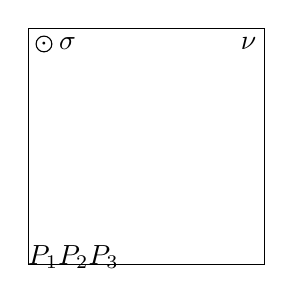
\begin{tikzpicture}
	\draw (0,0) rectangle (3,3);
	\node at (2.8,2.8) {$\nu$};
	\draw (0.2,2.8) circle (0.1);
	\node at (0.2,2.8) {$\cdot$};
	\node at (0.5,2.8) {$\sigma$};
	
	\tkzDefPoint(0.5,0.5){A}
	\tkzDefPoint(2.7,0.3){B}
	\tkzDefPoint(1.2,2.5){C}
	
	\tkzDrawPoints(A,B,C)
	\tkzLabelPoint[above](A){$P_1$}
	\tkzLabelPoint[above](B){$P_2$}
	\tkzLabelPoint[right](C){$P_3$}
	
	
\end{tikzpicture}
\end{minipage}
\begin{Answer}[ref = cmrot]
	Wir können uns zuerst überlegen, welche Bedingung die Winkelgeschwindigkeit $\omega$ erfüllen muss. Da sich die Körperabstände nicht ändern sollen, ist die potentielle Energie des Systems konstant. Da aber auch die Gesamtenergie erhalten bleibt, heißt das, dass auch die gesamte kinetische Energie konstant bleiben muss. Da sich aber bei einem starren Körper auch das Trägheitsmoment nicht ändern kann, heißt dass, das das System mit einer konstanten Winkelgeschwindigkeit $\omega$ rotieren muss.\\
	Wir geben nun die Positionen der drei Körper durch ihre Ortsvektoren $\mathbf{r_i}$ an. Dann wählen wir ein Koordinatensystem so, dass $\nu$ mit der $x-y-$Ebene zusammenfällt, und das $\sigma$ die $z-$Achse ist.\\
	In diesem Koordinatensystem ist der Schwerpunkt im Koordinatenursprung, es gilt also
	\begin{equation}\label{cmrot:com}
		\sum_{i=1}^{3} m_i\mathbf{r}_i = \mathbf{0}.
	\end{equation}
	Wir können jetzt o.B.d.A. die Kräfte betrachten, die auf den ersten Körper wirken. Das sind zum einen die Gravitationskräfte durch die Wechselwirkung mit Körper $2$ bzw. $3$ ($\mathbf{F}_{2}$ bzw. $\mathbf{F}_{3}$), als auch die im Inertialsystem wirkende Zentripetalkraft $\mathbf{F}_{z}$. Die Gravitationskräfte lassen sich durch die Seitenlängen im Dreieck ausdrücken:
	\begin{equation}\label{cmrot:grav}
		\mathbf{F}_2 = \frac{Gm_1m_2}{a_{1,2}^3}\left(\mathbf{r}_2-\mathbf{r}_1\right)~\mathrm{und}~\mathbf{F}_3 = \frac{Gm_1m_2}{a_{1,3}^3}\left(\mathbf{r}_3-\mathbf{r}_1\right).
	\end{equation}
	Die Zentripetalkraft ist gegeben durch
	\begin{equation}\label{cmrot:rot}
		\mathbf{F}_z = -m_1 \omega^2 \mathbf{r}_1,
	\end{equation}
	wobei $\omega$ die Winkelgeschwindigkeit ist.\\
	Im Kräftegleichgewicht, also bei konstater Rotation, muss nun gelten
	\begin{equation}\label{cmrot:fbal}
		\mathbf{F}_2 + \mathbf{F}_3 = \mathbf{F}_{z} \Rightarrow G \frac{m_1}{a_{1,2}^3} m_2 \mathbf{r}_2 + G \frac{m_1}{a_{1,3}}m_3\mathbf{r}_{3} + m_1 \mathbf{r}_1 \left(\omega^2 - \frac{Gm_2}{a_{1,2}^3} - \frac{Gm_3}{a_{1,3}}\right) = \mathbf{0}
	\end{equation}
	Gleichzeitig können wir \eqref{cmrot:com} umstellen nach
	\begin{equation}\label{cmrot:r2}
		m_2\mathbf{r}_2 = -m_1 \mathbf{r}_1 - m_3 \mathbf{r}_3.
	\end{equation}
	Wenn wir das jetzt wieder in \eqref{cmrot:fbal} einsetzen, kommen wir auf
	\begin{equation}\label{cmrot:ncl}
		\mathbf{r}_1m_1 \left(\omega^2 - \frac{Gm_2}{a_{1,2}^3} - \frac{Gm_3}{a_{1,3}^3} - \frac{Gm_1}{a_{1,2}^3}\right) + \mathbf{r}_{3} \left(\frac{1}{a_{1,3}^3} - \frac{1}{a_{1,2}^3} \right) = \mathbf{0}.
	\end{equation}
	Da nach Voraussetzung die Vektoren $\mathbf{r}_1$ aber nicht kolinear seien soll, ist die einzige Möglichkeit, dass eine Linearkombination von ihnen wie in \eqref{cmrot:ncl} den Nullvektor ergibt, dass die Koeffizienten null sind.\\
	Aus dem zweiten Term kommen wir jetzt auf 
	\begin{equation}\label{cmrot:el}
		\frac{1}{a_{1,3}^3} - \frac{1}{a_{1,2}^3} \overset{!}{=} 0 \Rightarrow a_{1,2} = a_{1,3}:= a.
	\end{equation}
	Der erste Term führt zu
	\begin{equation}
		\omega^2 a^3 = GM,
	\end{equation}
	mit $M = m_1+m_2+m_3$. \\
	Wenn wir den gleichen Spaß jetzt für die anderen beiden Körper machen, kommen wir darauf, dass alle drei Seiten gleich lang sein müssen, und die Bewegung nur dann als starrer Körper stattfinden kann, wenn alle drei mit konstanter Winkelgeschwindigkeit in Form eines gleichseitigen Dreiecks rotieren.
\end{Answer}

\begin{Exercise}[difficulty = 3, title = Komet, origin = {Auswahlwettbewerb IPhO 2007, 3. Runde}, label = cmcomet]
	Ein Komet bewegt sich auf einer parabolischen Bahn um die Sonne. Im sonnennächsten Punkt beträgt sein Abstand von der Sonne $\nicefrac{r_e}{3}$, wobei $r_e$ der Radius der als kreisförmig angenommenen Erdbahn ist. Alle anderen Wechselwirkungen als die mit der Sonne vernachlässigendend, wie lang ist die Zeit $\tau$, die sich der Komet innerhalb der Erdbahn befindet?\\
	\small{Es ist \begin{equation}
		\label{cmcomet:int}
		\int \frac{x}{\sqrt{x-a}}~dx = \frac{2}{3}\left(x+2a\right)\sqrt{x-a}\end{equation} für $x>a$ (Warum?).}
\end{Exercise}
\begin{Answer}[ref = cmcomet]
	Wir wissen, dass parabolische Bahnen zu einer Gesamtorbitenergie von $E = 0$ korrespondieren
	\begin{equation}\label{cmcomet:edef}
		  0 = \frac{\dot{r}^2 + r^2\dot{\varphi}^2}{2}- \frac{\Gamma}{r}.
	\end{equation}
	Hier bezeichnet $\varphi$ den Drehwinkel. Gleichzeitig wissen wir auch, dass der Betrag des Drehimpulses $\ell := \left|\mathbf{L}\right| = m r^2\dot{\varphi}$ konstant ist. Damit können wir die Winkelgeschwindigkeit durch $r$ und $\ell$ ausdrücken, und können die Energie nur in Abhängigkeit von $r$ und seinen Ableitungen darstellen
	\begin{equation}\label{cmcomet:effe}
		0 =\frac{\dot{r}^2}{2} + \frac{r^2}{2} \left(\frac{\ell}{mr^2}\right)^2 - \frac{\Gamma}{r} = \frac{\dot{r}^2}{2} + \frac{\ell^2}{2m^2r^2} - \frac{\Gamma}{r}.
	\end{equation}
	Das ist jetzt nur noch eine Differentialgleichung in $r\left(t\right)$, die wir zu lösen versuchen können. Bevor wir das machen, können wir noch schnell, auch mit \eqref{cmcomet:effe} den Drehimpuls ausrechnen, weil wir wissen, dass im Perihel $\dot{r} = 0$ gilt, und $r = \frac{r_e}{3}$:
	\begin{equation}\label{cmcomet:ldef}
		0 = \frac{\ell^2}{2m^2r^2} - \frac{\Gamma}{r} \Rightarrow \ell = m \sqrt{\frac{2}{3}\Gamma r}.
	\end{equation}
	Jetzt müssen wir wirklich nur noch die Differentialgleichung lösen. Wir stellen erstmal nach $\dot r$ um, bevor wir dann die Variablen trennen:
	\begin{equation*}
		\dot{r} = \pm \sqrt{\frac{\Gamma}{r} - \frac{\ell^2}{2m^2r^2}} =\pm \sqrt{2\Gamma}\sqrt{\frac{1}{r} -  \frac{r_e}{3r^2}}.
	\end{equation*}
	Mit $\dot{r} = \frac{dr}{dt}$ können wir jetzt einfach den Physiker-Umstell-Trick machen, und die Symmetrie des Problems nehmen, um uns über Vorzeichen keine Gedanken mehr machen zu müssen
	\begin{equation*}
		\int_0^\tau ~dt = \frac{2}{\sqrt{2\Gamma}}\int_{\frac{r_e}{3}}^{r_e} \frac{r}{\sqrt{r- \frac{r_e}{3}}}~dr.
	\end{equation*}
	Das Integral \eqref{cmcomet:int} ist zufällig das, was wir hier brauchen, und kommen so am Ende auf
	\begin{equation*}
		\boxed{\tau = \frac{20}{9} \cdot \sqrt{\frac{R^3}{3\Gamma}}.} 
	\end{equation*}
\end{Answer}
\begin{Exercise}[label = gravgrad, origin = {Auswahlwettbewerb IPhO 2013, 3. Runde}, title = {Gravity Gradient Stabilization}, difficulty = 5]
Wir betrachten einen Satelliten, der aus zwei Punktmassen $m_1$ und $m_2$ besteht, die durch einen massenlosen Strick der Länge $\ell$ verbunden sind. \\
Dieser Satellit befindet sich auf einer Kreisbahn um die Erde mit Radius $R$. Dabei zeigt er die Tendenz, sich aufzurichten, und um die sich einstellende Ruhelage zu oszillieren.\\
Bestimme die Frequenz $f$ dieser Schwingung.
\end{Exercise}
\begin{Answer}[ref = gravgrad]
	
\end{Answer}
\begin{Exercise}[label = phshift, title = Periheldrehung, difficulty = 5, origin = Aaron Wild]
	Wir betrachten ein Gravitationsfeld, was vom normalen Keplerschen um eine sehr kleine Pertubation $\delta U\left(r\right)$ abweicht:
	\begin{equation}\label{phshift:pot}
		U^\dagger\left(r\right) = U\left(r\right) + \delta U\left(r\right) = U\left(r\right)+\frac{\beta}{r^2}
	\end{equation}
	Das führt dazu, dass die elliptische Bahn, auf der ein Körper sich bewegt, nicht mehr geschlossen ist, sondern sich die Periapsis bei jeder Umdrehung um einen kleinen Winkel $\delta \varphi$ verschiebt. \\
	Bestimme $\delta \varphi$ in Abhängigkeit von den ursprünglichen Bahnparametern und $\beta$. \\
	Dabei kann ohne Beweis genutzt werden, dass bei einer solchen Änderung des Potentials der Drehimpulsvektor weiterhin konstant ist.
	
\end{Exercise}
\begin{Answer}[ref = phshift]
	Wir können die Änderung des Drehwinkels $\varphi$ über den Drehimpuls ausrechnen
	\begin{equation}\label{phshift:anmom}
		\ell = mr^2\frac{d\varphi}{dt} \Rightarrow d\varphi = \frac{\ell}{mr^2}\cdot dt.
	\end{equation}
	In der Energieerhaltung können wir jetzt für $\dot{\varphi}$ \eqref{phshift:anmom} einsetzen, und erhalten damit gleichzeitig einen Ausdruck für $dt$
	\begin{equation}\label{phshift:energy}
	E= \frac{m}{2}\left(\dot{r}^2 + r^2 \frac{\ell^2}{m^2r^4}\right) + U^{\dagger}\left(r\right) \Rightarrow dt = \frac{dr}{\sqrt{\frac{2}{m}\left[E-U^{\dagger}\left(r\right)\right] - \frac{\ell^2}{m^2r^2}}}.
	\end{equation}
	Das können wir jetzt in \eqref{phshift:anmom} einsetzen, um die Winkeländerung während eines Umlaufs auszurechnen
	\begin{equation}\label{phshift:anchange}
	\Delta \varphi = \int_{r_{min}}^{r_{max}} \frac{M}{r^2\sqrt{2m \left[E-U\left(r\right)\right] - \nicefrac{\ell^2}{r^2}}} ~dr.
	\end{equation}
	Es macht die Lösung jetzt einfacher, wenn man \eqref{phshift:anchange} in die Form
	\begin{equation}\label{phshift:anmom2}
		\Delta \varphi = -2\frac{\partial}{\partial \ell} \int_{r_{max}}^{r_{min}} \underbrace{\sqrt{2m\{E-\left[U\left(r\right) + \delta U\left(r\right)\right]\} - \frac{\ell^2}{r^2}}}_{:=I}~dr.
	\end{equation}
	zu bringen, wobei wir für $U^{\dagger}$ bereits \eqref{phshift:pot} eingesetzt haben.\\
	Wir können uns jetzt zu nutze machen, dass $\delta U\left(r\right)$ nur eine \textit{kleine} Störung der Bahn sein soll, um den Integranten aus \eqref{phshift:anmom2} durch eine Taylorerweiterung in der ersten Ordnung auszudrücken
	\begin{equation*}
		I \approx \sqrt{2m\left[E-U\left(r\right)\right] - \frac{\ell^2}{r^2}} + \frac{\partial}{\partial \delta U}\left(\sqrt{2m\{E-\left[U\left(r\right) + \delta U\left(r\right)\right]\} - \frac{\ell^2}{r^2}}\right) \cdot \delta U\left(r\right)
	\end{equation*}
	\begin{equation}\label{phshift:itay}
		\Rightarrow I \approx \sqrt{2m\left[E-U\left(r\right)\right] - \frac{\ell^2}{r^2}} - \frac{2m\delta U\left(r\right)}{\sqrt{2m\left[E-U\left(r\right) \right] - \frac{\ell^2}{r^2}}}
	\end{equation}
	Hier ist der erste Term jetzt genau der, den wir erwarten würden, wenn die Bahn nicht den kleinen zusätzlichen Potentialterm hätte. Und weil das Integral in \eqref{phshift:anmom2} über $I$ ja nach Summen getrennt durchgeführt werden kann, entspricht die Integration des ersten Terms aus \eqref{phshift:itay} genau der Bewegung auf der ungestörten Bahn, also $2\pi$. Denn wollen wir also gar nicht mehr betrachten ($\Delta \varphi = 2\pi + \delta \varphi$).\\
	Die gesuchte zusätzliche Winkeländerung $\delta\varphi$ ergibt sich also zu
	\begin{equation}\label{phshift:diffchange}
		\delta \varphi =\frac{\partial}{\partial \ell} \int_{r_{min}}^{r_{max}} \frac{2m\delta U\left(r\right)}{\sqrt{2m\left[E-U\left(r\right) \right] - \frac{\ell^2}{r^2}}}~dr.
	\end{equation}
	Weil wir schon den Effekt des Störpotentials in erster Ordnung durch die Taylorentwicklung einbezogen haben, ist es jetzt auch kein Problem mehr, wenn wir für $r\left(\varphi\right)$ einfach wieder die Lösung der ungestörten Bahngleichung annehmen. Damit ist haben wir jetzt auch eine Möglichkeit, $dr$ durch $d\varphi$ auszudrücken, und damit das Integral \eqref{phshift:diffchange} ordentlich auszuwerten.\\
	Dann können wir nämlich schreiben
	\begin{equation*}
		2m\left[E-U\left(r\right) \right] - \frac{\ell^2}{r^2} = 2m \left[\frac{1}{2}\left(m\dot{r}^2 + \frac{\ell^2}{mr^2}\right) + U\left(r\right) - U\left(r\right)\right] - \frac{\ell^2}{r^2}
	=	m^2\dot{r}^2.
	\end{equation*}
	Damit schreiben wir \eqref{phshift:diffchange} als
	\begin{equation}
		\delta \varphi = 2m\cdot \frac{\partial}{\partial \ell} \int_{r_{min}}^{r_{max}} \frac{ \delta U}{m\dot{r}}~dr =  2m\cdot \frac{\partial}{\partial \ell} \int_{r_{min}}^{r_{max}} \frac{\delta U}{m}dt.
	\end{equation}
	Jetzt können wir uns aber an \eqref{phshift:anmom} erinnern und den ganzen Spaß als
	\begin{equation}\label{phshift:subs}
		\delta \varphi = 2m\cdot \frac{\partial}{\partial \ell} \int_{0}^{\pi} \frac{\delta U}{m} \cdot \frac{mr^2}{\ell} ~d\varphi = \delta \varphi = 2m\cdot \frac{\partial}{\partial \ell}\left( \frac{1}{\ell} \int_{0}^{\pi} r^2\delta U d\varphi\right)
	\end{equation}
	schreiben.\\
	Weil nach \eqref{phshift:pot} das Störpotential dankenswerter Weise gerade $\delta U = \frac{\beta}{r^2}$ ist, kürzt sich $r^2$ und wir haben nur noch
	\begin{equation}
		\boxed{\delta \varphi = 2m\cdot \frac{\partial}{\partial \ell}\left( \frac{1}{\ell} \int_{0}^{\pi} \beta ~d\varphi\right) = -\frac{2\pi m\beta}{\ell^2}. 
			}
	\end{equation}
	
	
\end{Answer}

\begin{Exercise}[label = lso, difficulty = 3, origin = Aaron Wild, title = Schwarzschildmetrik]
	Die Bewegung eines Teilchens in der Schwarzschildmetrik\footnote[3]{Allgemein-relativistische Beschreibung der Gravitationswirkung eines ruhenden, sphärisch-symmetrischen Körpers.} kann durch ein effektives Potential der Form
	\begin{equation}\label{lso:ep}
		\tilde{U}\left(r\right) = \frac{mc^2}{2} \left(-\frac{r_s}{r} + \frac{a^2}{r^2} - \frac{r_sa^2}{r^3}\right).
	\end{equation}
	beschrieben werden. Dabei ist $r_s := \frac{2\Gamma}{c^2}$ der sog. \textit{Schwarzschildradius} und $ a := \frac{\ell}{mc}$ eine Referenzlänge.\\
	Die Gesamtenergie ist dann einfach
	\begin{equation}\label{lso:ene}
		E = \frac{m}{2}\dot{r}^2 + \tilde{U}\left(r\right).
	\end{equation}
	Finde die Radii, bei denen kreisförmige Orbits um den Zentralkörper möglich sind, sowie den Abstand $r_{isco}$ vom Zentralkörper, an dem der letzte stabile kreisförmige Orbit möglich ist. Dabei kann genutzt werden, dass für gewöhnlich $\frac{r_s}{a} \ll 1$ gilt.
\end{Exercise}
\begin{Answer}[ref = lso]
	Die notwendige Bedingung für stabile kreisförmige Orbits ist, dass die wirkende Gesamtkraft null ist. Die kriegen wir über die Ableitung von $\tilde{U}\left(r\right)$:
	\begin{equation}\label{lso:force}
		F = - \frac{d\tilde{U}}{dr} = - \frac{mc^2}{2r^4}\left(r_sr^2-2a^2r + 3r_sa^2\right) \overset{!}{=} 0.
	\end{equation}
	Wir können uns kurz überlegen, was die einzlnen Terme in \eqref{lso:force} bedeuten. Die ersten beiden kennen wir schon aus der klassischen Mechanik. Sie stehen respektive für das newtonsche Gravitationspotential, und den Beitrag durch die Drehimpulserhaltung zum effektiven Potential. Der dritte ist jetzt einfach der Beitrag durch relativistische Effekte, der, weil er proportional zu $c^{-2}$ ist, so klein ist, dass er bei normaler newtonscher Gravitation keinen sonderlich großen Einfluss hat.\\
	Wir können jetzt die quadratische Gleichung im geklammerten Term nach $r$ auflösen, um den größten und kleinsten Radius zu finden, an dem kreisförmige Orbits möglich sind:
	\begin{equation}\label{lso:quad}
		\frac{r^2}{r_s} - 2\frac{a^2}{r_s} + 3a^2 \overset{!}{=} 0 \Rightarrow r = \frac{a^2}{r_s}\left(1\pm \sqrt{1-\frac{3r_s^2}{a^2}}\right).
	\end{equation} 
	Wir können jetzt die zweite Ableitung von $\tilde{U}$ ausrechnen, um zu prüfen, welcher der Radii aus \eqref{lso:quad} stabil sind:
	\begin{equation}
		-\frac{d^2\tilde{U}}{dr^2} = \frac{2mc^2}{r^5} \left(r_sr^2 - 3a^2r+2r_sa^2\right).
	\end{equation}
	Wenn wir schön ist, dass wir in \eqref{lso:force} schon ein Teil des neuen Ausdrucks wieder finden, sodass wir leichter schreiben können
	\begin{equation}\label{lso:sd}
		-\frac{d\tilde{U}^2}{dr^2} =  \frac{2mc^2}{r^5} \left(r_sr^2 - 2a^2r + 3r_sa^2 -a^2r -a^2r_s\right) = \frac{-2mc^2a^2}{r^5}\left(r+r_s\right).
	\end{equation}
	Damit der Orbit stabil ist, muss jetzt $\frac{d\tilde{U}}{dr} >0$ gelten. Das ist in \eqref{lso:sd} nur für den äußeren Orbit $r_o$ der Fall, also der, der der Wahl des plus entspricht.\\
	Den letzten stabilen kreisförmigen Orbit haben wir, wenn $r_i = r_o$ gilt, damit also die Diskriminante in \eqref{lso:quad} gleich null ist. Dann gilt 
	\begin{equation}\label{lso:risco}\boxed{
		r_{isco} = \frac{a^2}{r_s} ~\mathrm{und}~a^2 = \frac{3}r_s^2 \Rightarrow r_{isco} = 3r_s,}
	\end{equation}
	was sogar unabhängig vom Schwarzschildradius ist.
\end{Answer}






\end{document}
